\documentclass[10pt]{article}

\usepackage{amsmath}

\newcommand{\myvec}[1]{\ensuremath{\begin{pmatrix}#1\end{pmatrix}}}

\newcommand{\mydet}[1]{\ensuremath{\begin{vmatrix}#1\end{vmatrix}}}

\newcommand{\solution}{\noindent \textbf{Solution: }}

\providecommand{\brak}[1]{\ensuremath{\left(#1\right)}}

\providecommand{\norm}[1]{\left\lVert#1\right\rVert}
\usepackage{graphicx}
\usepackage{float}

\let\vec\mathbf

\title{Coordinate Geometry}

\author{Aryam (aryamagrawal@sriprakashschools.com)}

\begin{document}

\maketitle

\section*{Class 10$^{th}$ Maths - Chapter 7}

This is Problem-6.3 from Exercise 7.1

\begin{enumerate}

\item Name the type of quadrilateral formed, if any, by the following points, and give reasons for your answer\\

(4,5), (7,6), (4,3),(1,2)\\

\solution\\

if $\brak{\vec{A}-\vec{B}}^{\top}\brak{\vec{D}-\vec{C}}=0$ then it is a parallelogram\\

$\myvec{-3&-1}\myvec{-3\\-1}$\\

-3(-3)+-1(-1)\\

9+1\\

10$\neq$=0\\

so, it is not a parallelogram\\

if $\brak{\vec{A}-\vec{C}}^{\top}\brak{\vec{B}-\vec{D}}=0$ then it is a rhombus\\

$\myvec{0& 2}{\myvec{6\\4}}$\\

0(6)+2(4)\\

0+8\\

8 $\neq$ 0\\

so it is not a rhombus\\

if $\brak{\vec{A}-\vec{D}}^{\top}\brak{\vec{A}-\vec{B}}=0$ then it is a square\\

$\myvec{3&3}{\myvec{-3\\-1}}$\\

3(-3)-3(-1)\\

-9+3\\

-6 $\neq$ 0\\

so, it is not a square\\

if $\brak{\vec{A}-\vec{B}}^{\top}\brak{\vec{B}-\vec{C}}=0$ then it is a rectangle\\

$\myvec{-3&-1}^{\top}{\myvec{3\\3}}$\\

-3(3)-1(3)\\

-9-3\\

-12$\neq$0\\

so, it is not a rectangle\\ 
\begin{figure}[H]
			\centering
			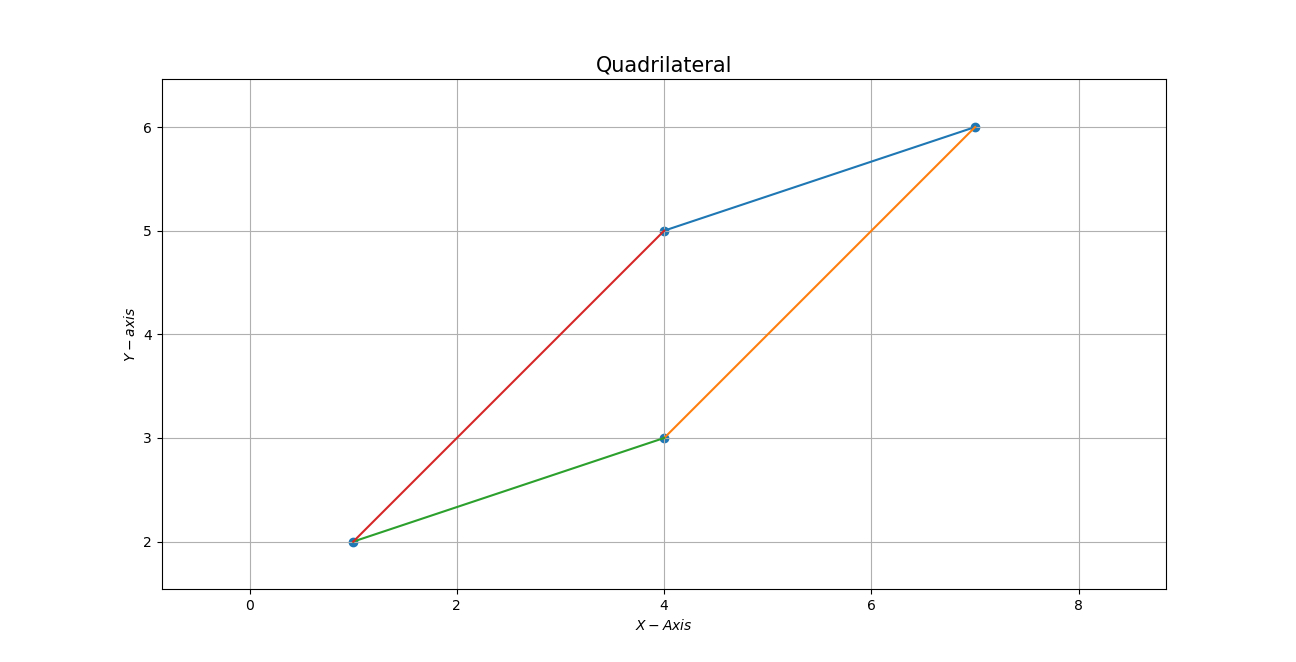
\includegraphics[width=\columnwidth]{figs/Figure_1}
			\caption{Quadrilateral ABCD}
			\label{fig:1}
		\end{figure}

\end{enumerate}

\end{document}
